% !TEX TS-program = pdflatex
% !TEX encoding = UTF-8 Unicode

% Example of the Memoir class, an alternative to the default LaTeX classes such as article and book, with many added features built into the class itself.

%\documentclass[12pt,a4paper]{memoir} % for a long document
\documentclass[12pt,a4paper,article]{memoir} % for a short document
\usepackage{hyperref}
\hypersetup{
    bookmarks=true,         % show bookmarks bar?
    pdftoolbar=true,        % show Acrobat’s toolbar?
    pdfmenubar=true,        % show Acrobat’s menu?
    pdffitwindow=false,     % window fit to page when opened
    pdftitle={BridgeBuilder Manual},    % title
    colorlinks=true,        % false: boxed links; true: colored links
    linkcolor=blue,         % color of internal links (change box color with linkbordercolor)
    citecolor=blue,         % color of links to bibliography
    filecolor=blue,         % color of file links
    urlcolor=cyan           % color of external links
}

\usepackage{graphicx} % support the \includegraphics command and options

\usepackage[utf8]{inputenc} % set input encoding to utf8
\usepackage{amssymb}
\usepackage{amsmath}
%\usepackage{stmaryrd}

\usepackage{listings}
\lstset{
	language=C++,
	basicstyle=\ttfamily,
	tabsize=2
}

% Don't forget to read the Memoir manual: memman.pdf

%%% Examples of Memoir customization
%%% enable, disable or adjust these as desired

%%% PAGE DIMENSIONS
% Set up the paper to be as close as possible to both A4 & letter:
\settrimmedsize{11in}{210mm}{*} % letter = 11in tall; a4 = 210mm wide
\setlength{\trimtop}{0pt}
\setlength{\trimedge}{\stockwidth}
\addtolength{\trimedge}{-\paperwidth}
\settypeblocksize{*}{\lxvchars}{1.618} % we want to the text block to have golden proportionals
\setulmargins{50pt}{*}{*} % 50pt upper margins
\setlrmargins{*}{*}{1.618} % golden ratio again for left/right margins
\setheaderspaces{*}{*}{1.618}
\checkandfixthelayout 
% This is from memman.pdf
\usepackage[margin=1.0in]{geometry}

%%% \maketitle CUSTOMISATION
% For more than trivial changes, you may as well do it yourself in a titlepage environment
%\pretitle{\begin{center}\sffamily\Huge\MakeUppercase}
\pretitle{\begin{center}\huge}
\posttitle{\par\end{center}\vskip 0.5em}

%%% ToC (table of contents) APPEARANCE
\maxtocdepth{subsection} % include subsections
\renewcommand{\cftchapterpagefont}{}
\renewcommand{\cftchapterfont}{}     % no bold!

%%% HEADERS & FOOTERS
\pagestyle{ruled} % try also: empty , plain , headings , ruled , Ruled , companion

%%% CHAPTERS
\chapterstyle{dash} % try also: default , section , hangnum , companion , article, demo

\renewcommand{\chaptitlefont}{\normalfont\Huge\center\scshape} % set sans serif chapter title font
\renewcommand{\chapnumfont}{\normalfont\Huge\scshape} % set sans serif chapter number font

%%% SECTIONS
\hangsecnum % hang the section numbers into the margin to match \chapterstyle{article}
\maxsecnumdepth{subsection} % number subsections

\setsecheadstyle{\normalfont\Large\raggedright\scshape} % set sans serif section font
%\setsubsecheadstyle{\large\sffamily\raggedright} % set sans serif subsection font

%% END Memoir customization

%%% TITLE
\title{\textbf{BridgeDesigner}}
\newcommand{\subtitle}{A Structural Design and Optimization Toolkit}
\author{\textit{created by Brian Doran Giffin}}
%\date{} % Delete this line to display the current date

\renewcommand{\maketitlehookb}{\centering\textsc{\subtitle}}

%%% BEGIN DOCUMENT
\begin{document}

\maketitle

\newpage

\tableofcontents* % the asterisk means that the contents itself isn't put into the ToC

\newpage

\chapter{Introduction}

BridgeDesigner is a structural design and optimization toolkit that was created with the intent of aiding student teams in designing efficient structures for entry into the National Student Steel Bridge Competition. The primary goal of BridgeDesigner is the complete automation of the CAD-to-analysis work-flow, while maintaining a fairly simple and straightforward implementation in Matlab which can be easily modified to address the specific needs of the user.

Previous efforts towards improving the CAD-to-analysis process focused on three major tasks: the creation of analysis-ready models from existing CAD drawing files; the assessment of a given model's structural efficiency according to simulated results provided by the chosen analysis software; and the optimization of a given structural design (usually just the selection of optimal tubing section sizes for some, or all structural members.) The first tools aimed at automating these tasks (\texttt{proto.Bridge}, \texttt{fore.Score}, and \texttt{re.Struct}, respectively) were written in Visual Basic, provided Excel spreadsheet user interfaces, and relied upon the AutoCAD and SAP2000 application programming interfaces (APIs) to send and receive model data between the relevant programs. However, these tools suffered largely from platform-specific issues: either the software itself was unavailable (or not widely available), or the APIs had been deprecated for certain student versions of the programs -- or, newer versions of the software employing different APIs produced run-time errors. All of these problems led to a great deal of effort on the part of users to get the design tools working on their personal computers, and for some, the tools were rendered inaccessible.

The BridgeDesigner structural design program aims to circumvent most of these issues, by avoiding the use of commercial APIs -- for both AutoCAD and SAP2000 -- altogether. Rather than retrieving drawing data from AutoCAD through API calls, BridgeDesigner is capable of processing files stored in the standardized \texttt{.dxf} drawing format, thereby allowing any version of AutoCAD (including student versions) to be used for automated design purposes. And, rather than interfacing with SAP2000, BridgeDesigner performs all of the relevant structural analysis computations internally using a simple and transparent structural finite element solver.

This document seeks to elaborate on the theoretical, implementational, and practical details regarding BridgeDesigner, in the hopes that it may see continued use, and possibly even open source development. Section \ref{sec:theory} discusses some of the theoretical background behind the analysis methods employed by BridgeDesigner, while section \ref{sec:implementation} addresses the implementational layout of the finite element and optimization tools. Section \ref{sec:usage} demonstrates how to use the BridgeDesigner toolkit through Matlab scripts, and provides some relevant examples of how to use the available features for design purposes.

\newpage

\chapter{Theoretical Development} \label{sec:theory}

This section summarizes some of the theoretical concepts underpinning the finite element method -- a computational approach commonly used to solve large problems in structural analysis. This discussion is intended to aid and inform prospective users or developers about the corresponding capabilities (and limitations) of the BridgeDesigner analysis toolkit, and of the structural finite element method, more generally.

\section{Overview of Structural Finite Element Methods}

The finite element method as applied to structural engineering problems (sometimes also referred to as ``matrix structural analysis'' in this setting) is an approach which seeks to directly determine the deformations experienced by a given structure via the solution of a discrete system of linear algebraic equations. These equations characterize two primary requirements on a given structure: force/moment equilibrium, and compatibility. In a discrete setting, the resulting finite element system of equations relates two fundamental quantities of interest: joint forces/moments, and joint displacements/rotations.

\subsection{Finite Element Equilibrium Equations}

The generic finite element problem is succinctly expressed as a balance of forces:
\begin{equation}
	\mathbf{f}^{\text{ext}} - \mathbf{f}^{\text{int}} = \mathbf{0},
\end{equation}
where $\mathbf{f}^{\text{ext}}$ is a vector of all \textit{externally applied} forces (and moments) acting on the joints of a structure, and $\mathbf{f}^{\text{int}}$ is the corresponding vector of \textit{internal} joint forces (and moments) induced by the internal stresses within all members comprising the structure. Henceforth, the term ``force'' (``displacement'') may be used to refer collectively to both forces and moments (displacements and rotations, respectively). For a structure to remain in equilibrium, the externally applied forces must balance with the internal forces, such that the \textit{net} force acting on each joint is equal to zero.

If we assume that the material relationship remains linearly elastic ($\sigma = E \varepsilon$), and that the displacements of the joints are relatively small in relation to the size of the structure, then we may express the vector $\mathbf{f}^{\text{int}}$ of internal forces as a direct linear function of the corresponding joint displacements $\mathbf{u}$ via:
\begin{equation}
	\mathbf{f}^{\text{int}} = \mathbf{K} \mathbf{u}.
	\label{eq:hookes_law}
\end{equation}
The ensuing matrix $\mathbf{K}$ is referred to as the ``stiffness matrix'' of the structure, which characterizes the (assumed linear) relationship between internal joint forces and joint displacements. Equation (\ref{eq:hookes_law}) may be regarded as a multi-dimensional generalization of Hooke's law. Thus, for a given set of externally applied forces $\mathbf{f}^{\text{ext}}$, the associated joint displacements may be determined by inverting the stiffness matrix:
\begin{equation}
	\mathbf{u} = \mathbf{K}^{-1} \mathbf{f}^{\text{ext}}.
\end{equation}
Once the joint displacements have been obtained by solving the finite element system of equations (above), the internal forces/stresses within all members of the structure may be computed as a post-processing procedure.

\subsection{Assembly of Finite Element Stiffness Matrices}

Most of the work involved in solving a matrix structural analysis problem boils down to two main procedures: computing and assembling the stiffness matrix of the structure as a whole, and solving the resulting linear system of equations. The second step is a linear algebra problem, easily solved by the numerical packages available in Matlab. The only difficult task that remains is the assembly of the structure's stiffness matrix.

To this end, it proves convenient to examine each member (or ``element'') of a given structure independently. In doing so, one may construct an ``element stiffness matrix'' $\mathbf{k}_e$, which relates the vector of displacements $\mathbf{u}_e$ applied to the ends of a single member, to the resulting joint forces $\mathbf{f}_e^{\text{int}}$ imposed by the element on the rest of the structure:
\begin{equation}
	\mathbf{f}_e^{\text{int}} = \mathbf{k}_e \mathbf{u}_e.
\end{equation}

\begin{figure}
	\centering
	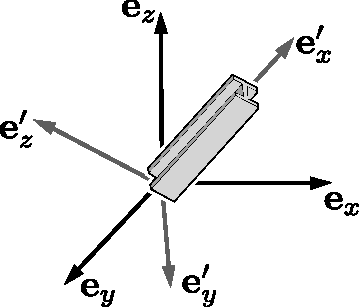
\includegraphics[width = 3in]{figures/element_coordinate_system.pdf}
	\caption{Depiction of the global (unprimed) and an element's local (primed) coordinate systems.}
	\label{fig:element_coordinate_system}
\end{figure}
In general, a given frame element may be oriented arbitrarily in 3-dimensional space, such that the axis of the member in question is not necessarily aligned with the ``global'' $x$-axis (refer to Figure \ref{fig:element_coordinate_system}.) For a variety of reasons, it proves convenient to define a ``local coordinate system'' for each element. Herein, quantities defined within an element's local coordinate system are denoted by a primed index (e.g. $\mathbf{u}'_e$ represents the vector of joint displacements oriented in the element's local coordinate system).

A traditional frame element possesses 2 joints: one at each of its end-points. In turn, each joint possesses 6 ``degrees of freedom:'' 3 translational displacements ($u_x'$, $u_y'$, $u_z'$) and 3 rotations ($\theta_x'$, $\theta_y'$, $\theta_z'$). These displacements and rotations are ``work-conjugated'' with the corresponding internal forces ($F_x'$, $F_y'$, $F_z'$) and moments ($M_x'$, $M_y'$, $M_z'$) acting at a given joint. 
\begin{figure}
	\centering
	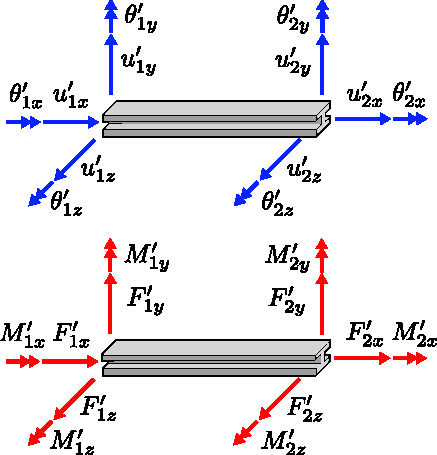
\includegraphics[width = 4.0in]{figures/frame.pdf}
	\caption{A representative 3D frame element oriented in its local coordinate system, with labeled joint displacements/rotations (top) and resulting internal joint forces/moments (bottom).}
	\label{fig:frame}
\end{figure}

The local stiffness matrix for a given frame element has dimensions of $12 \times 12$, accounting for the 6 degrees of freedom at each of its 2 joints (refer to Figure \ref{fig:frame}.) When expressed in the element's local coordinate system, the vectors of internal joint forces ${\mathbf{f}_e^{\text{int}}}'$ and joint displacements $\mathbf{u}_e'$ are related via
\begin{equation}
	{\mathbf{f}_e^{\text{int}}}' = \mathbf{k}_e' \mathbf{u}_e',
\end{equation}
where
\begin{equation}
	{\mathbf{f}_e^{\text{int}}}' \equiv \left\{ \begin{array}{cccccccccccc} F_{1x}' & F_{1y}' & F_{1z}' & M_{1x}' & M_{1y}' & M_{1z}' &  F_{2x}' & F_{2y}' & F_{2z}' & M_{2x}' & M_{2y}' & M_{2z}' \end{array} \right\}^T,
\end{equation}
\begin{equation}
	\mathbf{u}_e' \equiv \left\{ \begin{array}{cccccccccccc} u_{1x}' & u_{1y}' & u_{1z}' & \theta_{1x}' & \theta_{1y}' & \theta_{1z}' &  u_{2x}' & u_{2y}' & u_{2z}' & \theta_{2x}' & \theta_{2y}' & \theta_{2z}' \end{array} \right\}^T,
\end{equation}
\setlength\arraycolsep{-1pt}
\begin{equation}
	\mathbf{k}_e' \equiv \left[ \begin{array}{cccccccccccc} \frac{AE}{L} &  0 &  0 &  0 &  0 &  0 & -\frac{AE}{L} &  0 &  0 &  0 &  0 &  0 \\
                                                                  0 & \frac{12EI_z}{L^3} &  0 &  0 &  0 & \frac{6EI_z}{L^2} &  0 & -\frac{12EI_z}{L^3} &  0 &  0 &  0 & \frac{6EI_z}{L^2} \\
     						  0 &  0 & \frac{12EI_y}{L^3} &  0 & -\frac{6EI_y}{L^2} &  0 &  0 &  0 & -\frac{12EI_y}{L^3} &  0 & -\frac{6EI_y}{L^2} &  0 \\
     						0 &  0 &  0 & \frac{GJ}{L} &  0 &  0 &  0 &  0 &  0 & -\frac{GJ}{L} &  0 &  0 \\
    						 0 &  0 & -\frac{6EI_y}{L^2} &  0 & \frac{4EI_y}{L} &  0 &  0 &  0 & \frac{6EI_y}{L^2} &  0 & \frac{2EI_y}{L} &  0 \\
    						 0 & \frac{6EI_z}{L^2} &  0 &  0 &  0 & \frac{4EI_z}{L} &  0 & -\frac{6EI_z}{L^2} &  0 &  0 &  0 & \frac{2EI_z}{L} \\
    						-\frac{AE}{L} &  0 &  0 &  0 &  0 &  0 & \frac{AE}{L} &  0 &  0 &  0 &  0 &  0 \\
   						  0 & -\frac{12EI_z}{L^3} &  0 &  0 &  0 & -\frac{6EI_z}{L^2} &  0 & \frac{12EI_z}{L^3} &  0 &  0 &  0 & -\frac{6EI_z}{L^2} \\
   						  0 &  0 & -\frac{12EI_y}{L^3} &  0 & \frac{6EI_y}{L^2} &  0 &  0 &  0 & \frac{12EI_y}{L^3} &  0 & \frac{6EI_y}{L^2} &  0 \\
   						  0 &  0 &  0 & -\frac{GJ}{L} &  0 &  0 &  0 &  0 &  0 & \frac{GJ}{L} &  0 &  0 \\
    						 0 &  0 & -\frac{6EI_y}{L^2} &  0 & \frac{2EI_y}{L} &  0 &  0 &  0 & \frac{6EI_y}{L^2} &  0 & \frac{4EI_y}{L} &  0 \\
   						  0 & \frac{6EI_z}{L^2} &  0 &  0 &  0 & \frac{2EI_z}{L} &  0 & -\frac{6EI_z}{L^2} &  0 &  0 &  0 & \frac{4EI_z}{L} \end{array} \right].
\end{equation}
\setlength\arraycolsep{5pt} % (reset to default spacing)

The following quantities are herein defined, where the additional subscript $e$ is used later on to distinguish between properties belonging to differing elements:
\begin{itemize}
	\item[$E$]: Young's modulus of the material
	\item[$G$]: Shear modulus of the material ($G = \frac{E}{2(1+\nu)}$, with $\nu \equiv$ Poisson's ratio)
	\item[$A$]: Area of the element's cross-section
	\item[$I_y$]: Second moment of area about the element's local $y'$-axis
	\item[$I_z$]: Second moment of area about the element's local $z'$-axis
	\item[$J$]: Polar moment of area about the element's local $x'$-axis
	\item[$L$]: Length of the element
\end{itemize}

All that remains is to transform the element's stiffness matrix into the global coordinate system. To this end, let $\mathbf{Q}$ be defined as the $3\times3$ matrix which transforms the components of a vector $\mathbf{v}$ represented in the global coordinate system, into a vector $\mathbf{v}' = \mathbf{Q} \mathbf{v}$ represented in the element's local coordinate system, i.e.
\begin{equation}
  \mathbf{Q} = \left[ \begin{array}{ccc}
      \mathbf{e}'_x \cdot \mathbf{e}_x & \mathbf{e}'_x \cdot \mathbf{e}_y & \mathbf{e}'_x \cdot \mathbf{e}_z \\
      \mathbf{e}'_y \cdot \mathbf{e}_x & \mathbf{e}'_y \cdot \mathbf{e}_y & \mathbf{e}'_y \cdot \mathbf{e}_z \\
      \mathbf{e}'_z \cdot \mathbf{e}_x & \mathbf{e}'_z \cdot \mathbf{e}_y & \mathbf{e}'_z \cdot \mathbf{e}_z \end{array} \right].
\end{equation}
Further, let the following $12 \times 12$ ``element transformation matrix'' $\mathbf{T}$ be defined as
\begin{equation}
  \mathbf{T} = \left[ \begin{array}{cccc}
      \mathbf{Q} & \mathbf{0} & \mathbf{0} & \mathbf{0} \\
      \mathbf{0} & \mathbf{Q} & \mathbf{0} & \mathbf{0} \\
      \mathbf{0} & \mathbf{0} & \mathbf{Q} & \mathbf{0} \\
      \mathbf{0} & \mathbf{0} & \mathbf{0} & \mathbf{Q} \end{array} \right].
\end{equation}
It follows that
\begin{equation}
  {\mathbf{f}_e^{\text{int}}} = \mathbf{T}^T {\mathbf{f}_e^{\text{int}}}', \qquad \mathbf{u}_e = \mathbf{T}^T \mathbf{u}'_e, \qquad \mathbf{k}_e = \mathbf{T}^T \mathbf{k}'_e \mathbf{T}.
\end{equation}



%\section{Model Generation}

%\subsection{Geometry Processing}

%\subsubsection{Reading .dxf Files}


\section{Structural Optimization}

Within the context of the Steel Bridge competition, our goal is to design the most efficient structure possible, as determined by a pre-defined ``cost'' function:
\begin{equation}
	C(\Delta_{agg}, W) = f(\Delta_{agg}) + g(W),
\end{equation}
where $C(\Delta_{agg}, W)$ is the structural efficiency cost function which depnds on $W$ (the total weight of the structure) and $\Delta_{agg}$ (the total measured aggregate deflection). Typically,
\begin{equation}
	f(\Delta_{agg}) = c_\delta \Delta_{agg}
\end{equation}
and
\begin{equation}
	g(W) = c_w W
\end{equation}
where $c_w$ and $c_\delta$ are the associated costs per unit of weight and deflection, respectively.

The aggregate deflection $\Delta_{agg} (\mathbf{f})$ if a direct function of the applied loads $\mathbf{f}$ acting on the structure. In the setting of the Steel Bridge competition, there are usually multiple possible loading cases $\mathbf{f}_s$ where $s = 1, 2, \ldots, N_{cases}$, which will therefore result in multiple possible measurements of the aggregate deflection $\Delta_{agg} (\mathbf{f}_s)$. For this reason, one must consider the probabilistic average aggregate deflection for use in the aforementioned cost function, i.e.
\begin{equation}
	\Delta_{avg} = \sum_{s=1}^{N_{cases}} p(s) \Delta_{agg} (\mathbf{f}_s),
\end{equation}
where $p(s)$ denotes the probability measure that load case $s$ will occur during the competition. If all load cases have an equal chance of being selected, then we may consider the uniform probabilty distribution:
\begin{equation}
	\Delta_{avg} = \frac{1}{N_{cases}} \sum_{s=1}^{N_{cases}} \Delta_{agg} (\mathbf{f}_s).
\end{equation}

If we suppose that the joint displacements of the structure are obtained from $\mathbf{u}_s = \mathbf{K}^{-1} \mathbf{f}_s$ for a given load case $s$, then we may consider a ``measurement vector'' $\boldsymbol{\delta}_s$ which may be used to sample the deflections of specific joints in the structure (through a dot product with $\mathbf{u}_s$) to yield
\begin{equation}
	\Delta_{agg} (\mathbf{f}_s) = \boldsymbol{\delta}_s \cdot \mathbf{u}_s = \boldsymbol{\delta}_s \cdot \mathbf{K}^{-1} \mathbf{f}_s.
\end{equation}
It should be emphasized that both $\mathbf{f}_s$ and $\boldsymbol{\delta}_s$ are fixed quantities which are determined by the competition scoring criteria regarding loading and deflection measurement locations.

In comparison, the weight of the structure $W$ will remain unchanged regardless of which load case is selected, and may be computed via
\begin{equation}
	W = \sum_{e = 1}^{N_{members}} \rho A_e L_e
\end{equation}
where $\rho$ is the mass density of steel, and where $A_e$ and $L_e$ are the cross-sectional area and the length of a given member $e$.

For many years, both $c_w$ and $c_\delta$ were taken to be constants which did not depend upon $W$ or $\Delta_{agg}$. With the advent of the 2018 NSSBC rules, $c_\delta$ remains a constant scoring parameter, but the weight score $g(W)$ now depends implicitly upon the total weight $W$, such that
\setlength\arraycolsep{5pt}
\begin{equation}
	g(W) = \left\{ \begin{array}{cc} 0 & W < 120 \, \text{lbs} \\ \text{\$}5,000 (W - 120) & 120 \, \text{lbs} \leq W < 200 \, \text{lbs} \\ \text{\$}25,000 (W - 184) & W > 200 \, \text{lbs} \end{array} \right. .
\end{equation}
Alternatively, we may write
\begin{equation}
	g(W) = \langle \text{\$}5,000 (W - 120) \rangle + \langle \text{\$}20,000 (W - 200) \rangle,
\end{equation}
where $\langle x \rangle$ denotes the Macaulay bracket (or ramp) function, i.e. $\langle x \rangle = x$ if $x > 0$ and $\langle x \rangle = 0$ if $x \leq 0$.

The problem that we are faced with can be stated rather simply in mathematical terms:
\begin{equation}
	\min_{\mathbf{a}} C(\Delta_{agg}(\mathbf{a}), W(\mathbf{a}))
\end{equation}
where $\mathbf{a}$ represents a vector of generic structural parameters of interest (e.g. the spatial locations of certain joints, or the cross-sectional properties of various members). Considering the latter, suppose we were to contemplate a fixed structural configuration. We should like to select optimal tubing sections for each member, whose cross-sectional areas $A_e \, \forall e \in 1, \ldots, N_{members}$ will be taken as the minimizing parameters of interest. To solve for the optimal cross-sectional areas, we must first recognize that a minimum will be obtained when the derivative of the cost function with respect to each of the structural parameters is equal to zero:
\begin{equation}
	J_e = \frac{\partial C}{\partial A_e} = 0 \quad \forall e
\end{equation}
In mathematical terms, $J_e$ is referred to as the ``Jacobian'' of the cost function $C$.

The above will yield a system of simultaneous equations in the variables $A_e$, which when solved will yield a first-order approximation to the optimal section sizes. Because the cost function is in general a non-linear function of the parameters $A_e$, successive Newton iteration is required to achieve convergence to the final optimum values of $A_e$.

Considering the first partial derivative of $C$ with respect to the variables $A_e$, we obtain
\begin{equation}
	\frac{\partial C}{\partial A_e} = \frac{\partial f}{\partial A_e} + \frac{\partial g}{\partial A_e},
\end{equation}
and
\begin{equation}
	\frac{\partial f}{\partial A_e} = \frac{c_\delta}{N_{cases}} \sum_{s=1}^{N_{cases}} \boldsymbol{\delta}_s \cdot \frac{\partial \mathbf{K}^{-1}}{\partial A_e} \mathbf{f}_s, \qquad
	\frac{\partial g}{\partial A_e} = c_w (W) \rho L_e,
\end{equation}
where $c_w (W)$ is a piece-wise constant function of the total weight:
\begin{equation}
	c_w (W) = \left\{ \begin{array}{cc} 0 & W < 120 \, \text{lbs} \\ \text{\$}5,000 & 120 \, \text{lbs} \leq W < 200 \, \text{lbs} \\ \text{\$}25,000 & W > 200 \, \text{lbs} \end{array} \right. .
\end{equation}
Using the chain rule of differentiation, we may write
\begin{equation}
	\frac{\partial \mathbf{K}^{-1}}{\partial A_e} = \frac{\partial \mathbf{K}^{-1}}{\partial \mathbf{K}} \frac{\partial \mathbf{K}}{\partial A_e} = - \mathbf{K}^{-1} \mathbf{S}_e \mathbf{K}^{-1},
\end{equation}
where $\mathbf{S}_e = \partial \mathbf{K} / \partial A_e$ can be assembled from a single local element contribution $\mathbf{s}_e$:
\setlength\arraycolsep{-1pt}
\begin{equation}
	\mathbf{s}_e = \left[ \begin{array}{cccccccccccc} \frac{E}{L} &  0 &  0 &  0 &  0 &  0 & -\frac{E}{L} &  0 &  0 &  0 &  0 &  0 \\
                                                                  0 & \frac{12Er_g^2}{L^3} &  0 &  0 &  0 & \frac{6Er_g^2}{L^2} &  0 & -\frac{12Er_g^2}{L^3} &  0 &  0 &  0 & \frac{6Er_g^2}{L^2} \\
     						  0 &  0 & \frac{12Er_g^2}{L^3} &  0 & -\frac{6Er_g^2}{L^2} &  0 &  0 &  0 & -\frac{12Er_g^2}{L^3} &  0 & -\frac{6Er_g^2}{L^2} &  0 \\
     						0 &  0 &  0 & \frac{2Gr_g^2}{L} &  0 &  0 &  0 &  0 &  0 & -\frac{2Gr_g^2}{L} &  0 &  0 \\
    						 0 &  0 & -\frac{6Er_g^2}{L^2} &  0 & \frac{4Er_g^2}{L} &  0 &  0 &  0 & \frac{6Er_g^2}{L^2} &  0 & \frac{2Er_g^2}{L} &  0 \\
    						 0 & \frac{6Er_g^2}{L^2} &  0 &  0 &  0 & \frac{4Er_g^2}{L} &  0 & -\frac{6Er_g^2}{L^2} &  0 &  0 &  0 & \frac{2Er_g^2}{L} \\
    						-\frac{E}{L} &  0 &  0 &  0 &  0 &  0 & \frac{E}{L} &  0 &  0 &  0 &  0 &  0 \\
   						  0 & -\frac{12Er_g^2}{L^3} &  0 &  0 &  0 & -\frac{6Er_g^2}{L^2} &  0 & \frac{12Er_g^2}{L^3} &  0 &  0 &  0 & -\frac{6Er_g^2}{L^2} \\
   						  0 &  0 & -\frac{12Er_g^2}{L^3} &  0 & \frac{6Er_g^2}{L^2} &  0 &  0 &  0 & \frac{12Er_g^2}{L^3} &  0 & \frac{6Er_g^2}{L^2} &  0 \\
   						  0 &  0 &  0 & -\frac{2Gr_g^2}{L} &  0 &  0 &  0 &  0 &  0 & \frac{2Gr_g^2}{L} &  0 &  0 \\
    						 0 &  0 & -\frac{6Er_g^2}{L^2} &  0 & \frac{2Er_g^2}{L} &  0 &  0 &  0 & \frac{6Er_g^2}{L^2} &  0 & \frac{4Er_g^2}{L} &  0 \\
   						  0 & \frac{6Er_g^2}{L^2} &  0 &  0 &  0 & \frac{2Er_g^2}{L} &  0 & -\frac{6Er_g^2}{L^2} &  0 &  0 &  0 & \frac{4Er_g^2}{L} \end{array} \right],
\end{equation}
and where $r_g = \sqrt{I/A}$ represents the radius of gyration of the cross-section.

Ordinarily, we could puruse a solution to the above system of equations by taking the second derivative or ``Hessian'' of $C$, i.e.
\begin{equation}
	H_{ek} = \frac{\partial^2 C}{\partial A_e \partial A_k} = \frac{\partial^2 f}{\partial A_e \partial A_k} + \frac{\partial^2 g}{\partial A_e \partial A_k},
\end{equation}
\begin{equation}
	\frac{\partial^2 f}{\partial A_e \partial A_k} = \frac{c_\delta}{N_{cases}} \sum_{s=1}^{N_{cases}} \boldsymbol{\delta}_s \cdot \frac{\partial^2 \mathbf{K}^{-1}}{\partial A_e \partial A_k} \mathbf{f}_s, \qquad \frac{\partial^2 g}{\partial A_e \partial A_k} = 0,
\end{equation}
where
\begin{equation}
	\frac{\partial^2 \mathbf{K}^{-1}}{\partial A_e \partial A_k} = \mathbf{K}^{-1} \left[ \mathbf{S}_k \mathbf{K}^{-1} \mathbf{S}_e + \mathbf{S}_e \mathbf{K}^{-1} \mathbf{S}_k \right] \mathbf{K}^{-1},
\end{equation}
and
\begin{equation}
	\frac{\partial^2 \Delta_{agg} (\mathbf{f}_s)}{\partial A_e \partial A_k} = \boldsymbol{\gamma}_s \cdot \left[ \mathbf{S}_k \mathbf{K}^{-1} \mathbf{S}_e + \mathbf{S}_e \mathbf{K}^{-1} \mathbf{S}_k \right] \mathbf{u}_s = \boldsymbol{\Gamma}_{ks} \cdot \mathbf{K}^{-1} \mathbf{U}_{es} + \mathbf{U}_{ks} \cdot \mathbf{K}^{-1} \boldsymbol{\Gamma}_{es},
\end{equation}
We may then use the Hessian matrix to solve for the optimized cross-sectional areas within a Newton iteration procedure:
\begin{equation}
	\mathbf{A}_{i+1} = \mathbf{A}_{i} - \mathbf{H}_i^{-1} \mathbf{J}_i.
\end{equation}
There is a rather subtle issue at play here, however. Because of the inherent discontinuity in $c_w (W)$, we will most likely encounter convergence problems in our iteration procedure, particularly if the optimal weight of the structure lies at or near $W = 120$ or $W = 200$.

For this reason, we will assert the following postulate: \textit{the optimal weight of the structure should lie in the range $120 \leq W \leq 200$.} This raises an interesting mathematical challenge, as we must incorporate a constraint into our optimization procedure. We will choose to do so through the use of a single Karush-Kuhn-Tucker constraint, yielding the Lagrangian of the cost function:
\begin{equation}
	\Lambda(A_e, \mu) = C(A_e) + \mu (120 - W),
\end{equation}
where $\mu \geq 0$ is a complementary slack variable, such that $\mu = 0$ when $(120 - W) < 0$ and $\mu > 0$ when $(120 - W) \geq 0$. In this setting, we may consider the Jacobian of the Lagrangian:
\begin{equation}
	J_e = \frac{\partial \Lambda}{\partial A_e} = \frac{\partial C}{\partial A_e} - \mu \rho L_e = 0 \quad \forall e
\end{equation}
\begin{equation}
	J_\mu = \frac{\partial \Lambda}{\partial \mu} = 120 - \sum_{e = 1}^{N_{members}} \rho A_e L_e = 0
\end{equation}
and the corresponding Hessian:
\begin{equation}
	H_{ek} = \frac{\partial^2 \Lambda}{\partial A_e \partial A_k} = \frac{\partial^2 C}{\partial A_e \partial A_k},
\end{equation}
\begin{equation}
	H_{e\mu} = \frac{\partial^2 \Lambda}{\partial A_e \partial \mu} = - \rho L_e.
\end{equation}
The solution of the constrained minimum problem can be obtained from the saddle-point system of equations:
\setlength\arraycolsep{2pt}
\begin{equation}
	\left[ \begin{array}{cc} \mathbf{H}_{ek} & \mathbf{H}_{e\mu} \\ \mathbf{H}_{\mu k} & 0 \end{array} \right] \left\{ \begin{array}{c} \mathbf{A} \\ \mu \end{array} \right\} = \left\{ \begin{array}{c} \mathbf{J}_e \\ J_\mu \end{array} \right\}.
\end{equation}
In practice, this problem can be easily solved by first considering the unconstrained problem (assuming $\mu = 0$), checking whether the constraint $W > 120$ has been violated, and then optionally solving the above saddle-point problem to enforce the constraint (when $\mu > 0$).

The only problem that remains concerns the discrete nature of the available list of tubing sections. Consequently, it is recommended that the optimization be carried out in a continuous setting, and then mapped onto the discrete sub-space of available tubing section sizes via a closest-point projection method.

\section{Objective}

Define the following quanties:
\begin{itemize}
        \item[] $C$: the total cost of the structure
        \item[] $\Delta_s$: the aggregate deflection of the structure for load case $s$
        \item[] $W$: the total weight of the structure
        \item[] $c_\Delta$: the linear cost per unit of aggregate deflection
        \item[] $C_W$: the total cost of the overall structure's weight (an implicit function of $W$)
        \item[] $\mathbf{f}_s$: the net external loading on the structure for load case $s$
        \item[] $\mathbf{K}$: the stiffness matrix for the structure
        \item[] $\mathbf{u}_s$: the displacements of the structure for load case $s$
        \item[] $\mathbf{f}^*_s$: the virtual unit dummy force vector for load case $s$
        \item[] $\mathbf{u}^*_s$: the corresponding virtual displacement vector for load case $s$
        \item[] $p(s)$: the probability of occurance of load case $s$
        \item[] $\rho$: the density of steel
        \item[] $E$: the elastic modulus of steel
        \item[] $\nu$: the Poisson's ratio of steel
        \item[] $A_e$: the cross-sectional area of member $e$
        \item[] $I_e$: the moment of inertia of member $e$
        \item[] $J_e$: the polar moment of inertia of member $e$
        \item[] $r_e$: the radius of the section assigned to member $e$
        \item[] $t_e$: the wall thickness of the section assigned to member $e$
        \item[] $L_e$: the length of member $e$
        \item[] $\mathbf{a}$: the vector of all structure variables to be optimized
\end{itemize}

Mathematically, the Steel Bridge optimization problem is defined as: \textit{find the optimal values of all structural parameters $\mathbf{a}$ such that the overall cost $C$ of the structure is minimized, i.e.}
\begin{equation}
        \min_{\mathbf{a}} C(\mathbf{a})
\end{equation}
where
\begin{equation}
        C(\mathbf{a}) \equiv \sum_{s=1}^{N_s} p(s) \, C_{\Delta} (\Delta_s) + C_W (W),
\end{equation}
\begin{equation}
        \Delta_s (\mathbf{a}) \equiv \mathbf{f}^*_s \cdot \mathbf{K}^{-1} \cdot \mathbf{f}_s,
\end{equation}
\begin{equation}
        W (\mathbf{a}) \equiv \rho \sum_{e=1}^{N_e} A_e L_e.
\end{equation}
The stationarity of $C (\mathbf{a})$ implies that an optimal set of parameter values has been chosen, i.e.
\begin{equation}
        \mathbf{R} (\mathbf{a}) = \mathbf{0},
\end{equation}
where
\begin{equation}
        \mathbf{R} (\mathbf{a}) \equiv \frac{\partial C}{\partial \mathbf{a}} = \sum_{s=1}^{N_s} p(s) \, \frac{\partial C_\Delta}{\partial \Delta} \frac{\partial \Delta_s}{\partial \mathbf{a}} + \frac{\partial C_W}{\partial W} \frac{\partial W}{\partial \mathbf{a}},
\end{equation}
\begin{equation}
        \frac{\partial \Delta_s}{\partial \mathbf{a}} = \mathbf{f}^*_s \cdot \frac{\partial \mathbf{K}^{-1}}{\partial \mathbf{a}} \cdot \mathbf{f}_s,
\end{equation}
\begin{equation}
        \frac{\partial W}{\partial \mathbf{a}} = \rho \sum_{e=1}^{N_e} \left[ \frac{\partial A_e}{\partial \mathbf{a}} L_e + A_e \frac{\partial L_e}{\partial \mathbf{a}} \right],
\end{equation}
and
\begin{equation}
        \frac{\partial \mathbf{K}^{-1}}{\partial \mathbf{a}} = - \frac{1}{2} \left[ \mathbf{K}^{-1} \cdot \frac{\partial \mathbf{K}}{\partial \mathbf{a}} \cdot \mathbf{K}^{-1} + \left( \mathbf{K}^{-1} \cdot \frac{\partial \mathbf{K}}{\partial \mathbf{a}} \cdot \mathbf{K}^{-1} \right)^T \right].
\end{equation}
As a side note, it can be shown that any variation in the stiffness matrix $\delta \mathbf{K}$ due to a change in any structural parameter will always be symmetric, such that $\delta \mathbf{K} = (\delta \mathbf{K})^T$. This property permits the following simplification:
\begin{equation}
        \frac{\partial \mathbf{K}^{-1}}{\partial \mathbf{a}} = - \mathbf{K}^{-1} \cdot \frac{\partial \mathbf{K}}{\partial \mathbf{a}} \cdot \mathbf{K}^{-1},
\end{equation}
\begin{equation}
        \frac{\partial \Delta_s}{\partial \mathbf{a}} = - \mathbf{u}^*_s \cdot \frac{\partial \mathbf{K}}{\partial \mathbf{a}} \cdot \mathbf{u}_s.
\end{equation}

A Newton-Raphson iterative procedure may be used to solve for the optimal values of $\mathbf{a}$. Specifically, while $||\mathbf{R} (\mathbf{a}_k)|| > \epsilon$, compute an updated set of parameter values $\mathbf{a}_{k+1}$ via
\begin{equation}
        \mathbf{a}_{k+1} = \mathbf{a}_k - \left[ \mathbf{J} (\mathbf{a}_k) \right]^{-1} \mathbf{R} (\mathbf{a}_k),
\end{equation}
where
\begin{equation}
        \mathbf{J} (\mathbf{a}) \equiv \frac{\partial^2 C}{\partial \mathbf{a} \otimes \partial \mathbf{a}},
\end{equation}
\begin{equation}
        \frac{\partial^2 C}{\partial \mathbf{a} \otimes \partial \mathbf{a}} = \sum_{s=1}^{N_s} p(s) \, \frac{\partial^2 \Delta_s}{\partial \mathbf{a} \otimes \partial \mathbf{a}} + \frac{\partial C_W}{\partial W} \frac{\partial^2 W}{\partial \mathbf{a} \otimes \partial \mathbf{a}} + \frac{\partial^2 C_W}{\partial W^2} \left[ \frac{\partial W}{\partial \mathbf{a}} \otimes \frac{\partial W}{\partial \mathbf{a}} \right],
\end{equation}
\begin{equation}
        \frac{\partial^2 \Delta_s}{\partial a_i \, \partial a_j} = \mathbf{f}^*_s \cdot \frac{\partial^2 \mathbf{K}^{-1}}{\partial a_i \, \partial a_j} \cdot \mathbf{f}_s,
\end{equation}
\begin{equation}
        \frac{\partial^2 W}{\partial \mathbf{a} \otimes \partial \mathbf{a}} = \rho \sum_{e=1}^{N_e} \left[ \frac{\partial^2 A_e}{\partial \mathbf{a} \otimes \partial \mathbf{a}} L_e + \frac{\partial A_e}{\partial \mathbf{a}} \otimes \frac{\partial L_e}{\partial \mathbf{a}} + \frac{\partial L_e}{\partial \mathbf{a}} \otimes \frac{\partial A_e}{\partial \mathbf{a}} + A_e \frac{\partial^2 L_e}{\partial \mathbf{a} \otimes \partial \mathbf{a}} \right],
\end{equation}
and
\begin{eqnarray}
        \frac{\partial^2 \mathbf{K}^{-1}}{\partial a_i \, \partial a_j} = \mathbf{K}^{-1} \cdot \left[ \frac{\partial \mathbf{K}}{\partial a_i} \cdot \mathbf{K}^{-1} \cdot \frac{\partial \mathbf{K}}{\partial a_j} + \frac{\partial \mathbf{K}}{\partial a_j} \cdot \mathbf{K}^{-1} \cdot \frac{\partial \mathbf{K}}{\partial a_i} - \frac{\partial^2 \mathbf{K}}{\partial a_i \, \partial a_j} \right] \cdot \mathbf{K}^{-1},
\end{eqnarray}
\begin{equation}
        \frac{\partial^2 \Delta_s}{\partial a_i \, \partial a_j} = \mathbf{u}^*_s \cdot \left[ \frac{\partial \mathbf{K}}{\partial a_i} \cdot \mathbf{K}^{-1} \cdot \frac{\partial \mathbf{K}}{\partial a_j} + \frac{\partial \mathbf{K}}{\partial a_j} \cdot \mathbf{K}^{-1} \cdot \frac{\partial \mathbf{K}}{\partial a_i} - \frac{\partial^2 \mathbf{K}}{\partial a_i \, \partial a_j} \right] \cdot \mathbf{u}_s.
\end{equation}
Let the following terms be defined:
\begin{equation}
  \left. \frac{\partial \mathbf{f}_s}{\partial a_i} \right|_{\mathbf{u}_s} = \frac{\partial \mathbf{K}}{\partial a_i} \cdot \mathbf{u}_s, \quad
  \left. \frac{\partial^2 \Delta_s}{\partial a_i \, \partial a_j} \right|_{\mathbf{u}_s, \mathbf{u}^*_s} = \mathbf{u}^*_s \cdot \frac{\partial^2 \mathbf{K}}{\partial a_i \, \partial a_j} \cdot \mathbf{u}_s.
\end{equation}
Thus:
\begin{equation}
  \frac{\partial^2 \Delta_s}{\partial a_i \, \partial a_j} = \left. \frac{\partial \mathbf{f}^*_s}{\partial a_i} \right|_{\mathbf{u}^*_s} \cdot \mathbf{K}^{-1} \cdot \left. \frac{\partial \mathbf{f}_s}{\partial a_j} \right|_{\mathbf{u}_s} + \left. \frac{\partial \mathbf{f}^*_s}{\partial a_j} \right|_{\mathbf{u}^*_s} \cdot \mathbf{K}^{-1} \cdot \left. \frac{\partial \mathbf{f}_s}{\partial a_i} \right|_{\mathbf{u}_s} - \left. \frac{\partial^2 \Delta_s}{\partial a_i \, \partial a_j} \right|_{\mathbf{u}_s, \mathbf{u}^*_s}.
\end{equation}

In general, $\mathbf{J} (\mathbf{a})$ will be a dense matrix. Thus, for sufficiently large problems, it may be more efficient to move away from a gradient-based optimization method.

\section{Section Property Derivatives}

Given a hollow circular section with outer radius $r$ and wall thickness $t$, the section properties may be written as
\begin{equation}
  A = \pi \left[ r^2 - (r-t)^2 \right], \quad I = \frac{\pi}{4} \left[ r^4 - (r-t)^4 \right], \quad I \equiv I_y = I_z = \frac{J}{2}.
\end{equation}
The first and second (including mixed) partial derivatives of $A$ and $I$ with respect to $r$ and $t$ are:
\begin{equation}
  \left[ \begin{array}{cc} A_{,r} & I_{,r} \\ A_{,t} & I_{,t} \end{array} \right] = \left[ \begin{array}{cc} 2 \pi t & \pi \left[ r^3 - (r-t)^3 \right] \\ 2 \pi (r-t) & \pi (r - t)^3 \end{array} \right], \quad
  \left[ \begin{array}{cc} A_{,rr} & I_{,rr} \\ A_{,rt} & I_{,rt} \\ A_{,tt} & I_{,tt} \end{array} \right] = \left[ \begin{array}{cc} 0 & 3 \pi \left[ r^2 - (r-t)^2 \right] \\ 2 \pi & 3 \pi (r-t)^2 \\ - 2 \pi & - 3 \pi (r-t)^2 \end{array} \right].
\end{equation}

\section{Element Geometry Derivatives}

\begin{equation}
        \frac{\partial L_e}{\partial \mathbf{a}} = \boldsymbol{\lambda}_e \cdot \left[ \frac{\partial \mathbf{X}_2^e}{\partial \mathbf{a}} - \frac{\partial \mathbf{X}_1^e}{\partial \mathbf{a}} \right], \qquad \boldsymbol{\lambda}_e = \frac{\mathbf{X}_2^e - \mathbf{X}_1^e}{L_e}.
\end{equation}

\section{Element Stiffness Matrix}

\begin{equation}
  \mathbf{f}_e = \left\{ \begin{array}{cccccccccccc} F_{x1} & F_{y1} & F_{z1} & M_{x1} & M_{y1} & M_{z1} & F_{x2} & F_{y2} & F_{z2} & M_{x2} & M_{y2} & M_{z2} \end{array} \right\}^T,
\end{equation}
\begin{equation}
\mathbf{u}_e = \left\{ \begin{array}{cccccccccccc} u_{x1} & u_{y1} & u_{z1} & \theta_{x1} & \theta_{y1} & \theta_{z1} & u_{x2} & u_{y2} & u_{z2} & \theta_{x2} & \theta_{y2} & \theta_{z2} \end{array} \right\}^T,
\end{equation}
\begin{equation}
  \mathbf{f}_e = \mathbf{T}^T \mathbf{f}'_e,
\end{equation}
\begin{equation}
  \mathbf{u}'_e = \mathbf{T} \mathbf{u}_e,
\end{equation}
\begin{equation}
  \mathbf{k}_e = \mathbf{T}^T \mathbf{k}'_e \mathbf{T},
\end{equation}
\begin{equation}
  \mathbf{T} = \left[ \begin{array}{cccc}
      \mathbf{Q} & \mathbf{0} & \mathbf{0} & \mathbf{0} \\
      \mathbf{0} & \mathbf{Q} & \mathbf{0} & \mathbf{0} \\
      \mathbf{0} & \mathbf{0} & \mathbf{Q} & \mathbf{0} \\
      \mathbf{0} & \mathbf{0} & \mathbf{0} & \mathbf{Q} \end{array} \right],
\end{equation}
\begin{equation}
  \mathbf{Q} = \left[ \begin{array}{ccc}
      \mathbf{e}'_1 \cdot \mathbf{e}_1 & \mathbf{e}'_1 \cdot \mathbf{e}_2 & \mathbf{e}'_1 \cdot \mathbf{e}_3 \\
      \mathbf{e}'_2 \cdot \mathbf{e}_1 & \mathbf{e}'_2 \cdot \mathbf{e}_2 & \mathbf{e}'_2 \cdot \mathbf{e}_3 \\
      \mathbf{e}'_3 \cdot \mathbf{e}_1 & \mathbf{e}'_3 \cdot \mathbf{e}_2 & \mathbf{e}'_3 \cdot \mathbf{e}_3 \end{array} \right],
\end{equation}
\begin{equation}
  \mathbf{k}'_e = \left[ \begin{array}{cccccccccccc}
      k'_{1,1} & 0 & 0 & 0 & 0 & 0 & k'_{1,7} & 0 & 0 & 0 & 0 & 0 \\
      0 & k'_{2,2} & 0 & 0 & 0 & k'_{2,6} & 0 & k'_{2,8} & 0 & 0 & 0 & k'_{2,12} \\
      0 & 0 & k'_{3,3} & 0 & k'_{3,5} & 0 & 0 & 0 & k'_{3,9} & 0 & k'_{3,11} & 0 \\
      0 & 0 & 0 & k'_{4,4} & 0 & 0 & 0 & 0 & 0 & k'_{4,10} & 0 & 0 \\
      0 & 0 & k'_{5,3} & 0 & k'_{5,5} & 0 & 0 & 0 & k'_{5,9} & 0 & k'_{5,11} & 0 \\
      0 & k'_{6,2} & 0 & 0 & 0 & k'_{6,6} & 0 & k'_{6,8} & 0 & 0 & 0 & k'_{6,12} \\
      k'_{7,1} & 0 & 0 & 0 & 0 & 0 & k'_{7,7} & 0 & 0 & 0 & 0 & 0 \\
      0 & k'_{8,2} & 0 & 0 & 0 & k'_{8,6} & 0 & k'_{8,8} & 0 & 0 & 0 & k'_{8,12} \\
      0 & 0 & k'_{9,3} & 0 & k'_{9,5} & 0 & 0 & 0 & k'_{9,9} & 0 & k'_{9,11} & 0 \\
      0 & 0 & 0 & k'_{10,4} & 0 & 0 & 0 & 0 & 0 & k'_{10,10} & 0 & 0 \\
      0 & 0 & k'_{11,3} & 0 & k'_{11,5} & 0 & 0 & 0 & k'_{11,9} & 0 & k'_{11,11} & 0 \\
      0 & k'_{12,2} & 0 & 0 & 0 & k'_{12,6} & 0 & k'_{12,8} & 0 & 0 & 0 & k'_{12,12} 
      \end{array} \right],
\end{equation}
\begin{equation}
  \tilde{\mathbf{k}}_{u'_x}^{F'_x} = \frac{1}{A} \left[ \begin{array}{cc}
      k'_{1,1} & k'_{1,7} \\ k'_{7,1} & k'_{7,7} \end{array} \right] = \frac{E}{L} \left[ \begin{array}{cc}
      +1 & -1 \\ -1 & +1 \end{array} \right],
\end{equation}
\begin{equation}
  \tilde{\mathbf{k}}_{\theta'_x}^{M'_x} = \frac{1}{J} \left[ \begin{array}{cc}
      k'_{4,4} & k'_{4,10} \\ k'_{10,4} & k'_{10,10} \end{array} \right] = \frac{E}{2(1+\nu)L} \left[ \begin{array}{cc}
      +1 & -1 \\ -1 & +1 \end{array} \right],
\end{equation}
\begin{equation}
  \tilde{\mathbf{k}}_{u'_y}^{F'_y} = \frac{1}{I_z} \left[ \begin{array}{cc}
      k'_{2,2} & k'_{2,8} \\ k'_{8,2} & k'_{8,8} \end{array} \right] = \frac{12E}{L^3} \left[ \begin{array}{cc}
      +1 & -1 \\ -1 & +1 \end{array} \right], \quad
  \tilde{\mathbf{k}}_{\theta'_z}^{F'_y} = \frac{1}{I_z} \left[ \begin{array}{cc}
      k'_{2,6} & k'_{2,12} \\ k'_{8,6} & k'_{8,12} \end{array} \right] = \frac{6E}{L^2} \left[ \begin{array}{cc}
      +1 & +1 \\ -1 & -1 \end{array} \right],
\end{equation}
\begin{equation}
  \tilde{\mathbf{k}}_{\theta'_z}^{M'_z} = \frac{1}{I_z} \left[ \begin{array}{cc}
      k'_{6,6} & k'_{6,12} \\ k'_{12,6} & k'_{12,12} \end{array} \right] = \frac{2E}{L} \left[ \begin{array}{cc}
      +2 & +1 \\ +1 & +2 \end{array} \right], \quad
  \tilde{\mathbf{k}}_{u'_y}^{M'_z} = \frac{1}{I_z} \left[ \begin{array}{cc}
      k'_{6,2} & k'_{6,8} \\ k'_{12,2} & k'_{12,8} \end{array} \right] = \frac{6E}{L^2} \left[ \begin{array}{cc}
      +1 & -1 \\ +1 & -1 \end{array} \right],
\end{equation}
\begin{equation}
  \tilde{\mathbf{k}}_{u'_z}^{F'_z} = \frac{1}{I_y} \left[ \begin{array}{cc}
      k'_{3,3} & k'_{3,9} \\ k'_{9,3} & k'_{9,9} \end{array} \right] = \frac{12E}{L^3} \left[ \begin{array}{cc}
      +1 & -1 \\ -1 & +1 \end{array} \right], \quad
  \tilde{\mathbf{k}}_{\theta'_y}^{F'_z} = \frac{1}{I_y} \left[ \begin{array}{cc}
      k'_{3,5} & k'_{3,11} \\ k'_{9,5} & k'_{9,11} \end{array} \right] = \frac{6E}{L^2} \left[ \begin{array}{cc}
      -1 & -1 \\ +1 & +1 \end{array} \right],
\end{equation}
\begin{equation}
  \tilde{\mathbf{k}}_{\theta'_y}^{M'_y} = \frac{1}{I_y} \left[ \begin{array}{cc}
      k'_{5,5} & k'_{5,11} \\ k'_{11,5} & k'_{11,11} \end{array} \right] = \frac{2E}{L} \left[ \begin{array}{cc}
      +2 & +1 \\ +1 & +2 \end{array} \right], \quad
  \tilde{\mathbf{k}}_{u'_z}^{M'_y} = \frac{1}{I_y} \left[ \begin{array}{cc}
      k'_{5,3} & k'_{5,9} \\ k'_{11,3} & k'_{11,9} \end{array} \right] = \frac{6E}{L^2} \left[ \begin{array}{cc}
      -1 & +1 \\ -1 & +1 \end{array} \right],
\end{equation}
\begin{equation}
  \mathbf{f}_{F'_x} = \left\{ \begin{array}{c} F'_{x1} \\ F'_{x2} \end{array} \right\}, \quad 
  \mathbf{u}_{u'_x} = \left\{ \begin{array}{c} u'_{x1} \\ u'_{x2} \end{array} \right\}, \quad
  \mathbf{f}_{F'_x} = A \left( \tilde{\mathbf{k}}_{u'_x}^{F'_x} \mathbf{u}_{u'_x} \right),
\end{equation}
\begin{equation}
  \mathbf{f}_{M'_x} = \left\{ \begin{array}{c} M'_{x1} \\ M'_{x2} \end{array} \right\}, \quad 
  \mathbf{u}_{\theta'_x} = \left\{ \begin{array}{c} \theta'_{x1} \\ \theta'_{x2} \end{array} \right\}, \quad
  \mathbf{f}_{M'_x} = J \left( \tilde{\mathbf{k}}_{\theta'_x}^{M'_x} \mathbf{u}_{\theta'_x} \right),
\end{equation}
\begin{equation}
  \mathbf{f}_{F'_y} = \left\{ \begin{array}{c} F'_{y1} \\ F'_{y2} \end{array} \right\}, \quad 
  \mathbf{u}_{u'_y} = \left\{ \begin{array}{c} u'_{y1} \\ u'_{y2} \end{array} \right\}, \quad
  \mathbf{f}_{M'_z} = \left\{ \begin{array}{c} M'_{z1} \\ M'_{z2} \end{array} \right\}, \quad 
  \mathbf{u}_{\theta'_z} = \left\{ \begin{array}{c} \theta'_{z1} \\ \theta'_{z2} \end{array} \right\},
\end{equation}
\begin{equation}
  \left\{ \begin{array}{c} \mathbf{f}_{F'_y} \\ \mathbf{f}_{M'_z} \end{array} \right\} = I_z \left[ \begin{array}{cc} \tilde{\mathbf{k}}_{u'_y}^{F'_y} & \tilde{\mathbf{k}}_{\theta'_z}^{F'_y} \\ \tilde{\mathbf{k}}_{u'_y}^{M'_z} & \tilde{\mathbf{k}}_{\theta'_z}^{M'_z} \end{array} \right] \left\{ \begin{array}{c} \mathbf{u}_{u'_y} \\ \mathbf{u}_{\theta'_z} \end{array} \right\},
\end{equation}
\begin{equation}
  \mathbf{f}_{F'_z} = \left\{ \begin{array}{c} F'_{z1} \\ F'_{z2} \end{array} \right\}, \quad 
  \mathbf{u}_{u'_z} = \left\{ \begin{array}{c} u'_{z1} \\ u'_{z2} \end{array} \right\}, \quad
  \mathbf{f}_{M'_y} = \left\{ \begin{array}{c} M'_{y1} \\ M'_{y2} \end{array} \right\}, \quad 
  \mathbf{u}_{\theta'_y} = \left\{ \begin{array}{c} \theta'_{y1} \\ \theta'_{y2} \end{array} \right\},
\end{equation}
\begin{equation}
  \left\{ \begin{array}{c} \mathbf{f}_{F'_z} \\ \mathbf{f}_{M'_y} \end{array} \right\} = I_y \left[ \begin{array}{cc} \tilde{\mathbf{k}}_{u'_z}^{F'_z} & \tilde{\mathbf{k}}_{\theta'_y}^{F'_z} \\ \tilde{\mathbf{k}}_{u'_z}^{M'_y} & \tilde{\mathbf{k}}_{\theta'_y}^{M'_y} \end{array} \right] \left\{ \begin{array}{c} \mathbf{u}_{u'_z} \\ \mathbf{u}_{\theta'_y} \end{array} \right\},
\end{equation}
\begin{equation}
  \Delta^e_{,A} = \mathbf{u}^*_{u'_x} \cdot \tilde{\mathbf{k}}_{u'_x}^{F'_x} \mathbf{u}_{u'_x}, \quad
  \Delta^e_{,J} = \mathbf{u}^*_{\theta'_x} \cdot \tilde{\mathbf{k}}_{\theta'_x}^{M'_x} \mathbf{u}_{\theta'_x},
\end{equation}
\begin{equation}
  \Delta^e_{,I_z} = \left\{ \begin{array}{cc} \mathbf{u}^*_{u'_y} & \mathbf{u}^*_{\theta'_z} \end{array} \right\} \cdot \left[ \begin{array}{cc} \tilde{\mathbf{k}}_{u'_y}^{F'_y} & \tilde{\mathbf{k}}_{\theta'_z}^{F'_y} \\ \tilde{\mathbf{k}}_{u'_y}^{M'_z} & \tilde{\mathbf{k}}_{\theta'_z}^{M'_z} \end{array} \right] \left\{ \begin{array}{c} \mathbf{u}_{u'_y} \\ \mathbf{u}_{\theta'_z} \end{array} \right\}, \quad
  \Delta^e_{,I_y} = \left\{ \begin{array}{cc} \mathbf{u}^*_{u'_z} & \mathbf{u}^*_{\theta'_y} \end{array} \right\} \cdot \left[ \begin{array}{cc} \tilde{\mathbf{k}}_{u'_z}^{F'_z} & \tilde{\mathbf{k}}_{\theta'_y}^{F'_z} \\ \tilde{\mathbf{k}}_{u'_z}^{M'_y} & \tilde{\mathbf{k}}_{\theta'_y}^{M'_y} \end{array} \right] \left\{ \begin{array}{c} \mathbf{u}_{u'_z} \\ \mathbf{u}_{\theta'_y} \end{array} \right\},
\end{equation}
\begin{equation}
  \Delta^e = \mathbf{u}^*_e \cdot \mathbf{f}_e = \mathbf{u}'^{*}_e \cdot \mathbf{f}'_e = \Delta^e_{,A} A + \Delta^e_{,J} J + \Delta^e_{,I_z} I_z + \Delta^e_{,I_y} I_y.
\end{equation}

For hollow circular (or square) cross-sections where $I \equiv I_y = I_z = \frac{J}{2}$:
\begin{equation}
  \Delta^e = \Delta^e_{,A} A + \Delta^e_{,I} I, \quad \Delta^e_{,I} = 2 \Delta^e_{,J} + \Delta^e_{,I_z} + \Delta^e_{,I_y},
\end{equation}
For hollow circular cross-sections, the first and second (including mixed) partial derivatives of $\Delta^e$ with respect to $r$ and $t$ are:
\begin{equation}
  \left\{ \begin{array}{c} \Delta^e_{,r} \\ \Delta^e_{,t} \end{array} \right\} = \left[ \begin{array}{cc} A_{,r} & I_{,r} \\ A_{,t} & I_{,t} \end{array} \right] \left\{ \begin{array}{c} \Delta^e_{,A} \\ \Delta^e_{,I} \end{array} \right\}, \quad
  \left\{ \begin{array}{c} \Delta^e_{,rr} \\ \Delta^e_{,rt} \\ \Delta^e_{,tt} \end{array} \right\} = \left[ \begin{array}{cc} A_{,rr} & I_{,rr} \\ A_{,rt} & I_{,rt}  \\ A_{,tt} & I_{,tt} \end{array} \right] \left\{ \begin{array}{c} \Delta^e_{,A} \\ \Delta^e_{,I} \end{array} \right\}.
\end{equation}
The resulting mixed partial derivatives with respect to $\mathbf{u}'_e$ and $\mathbf{u}'^*_e$ are:
\begin{equation}
  \mathbf{f}'^*_{e,A} = \mathbf{k}'_{,A} \mathbf{u}'^*_e, \quad
  \mathbf{f}'^*_{e,I} = 2 \mathbf{f}'^*_{e,J} + \mathbf{f}'^*_{e,I_z} + \mathbf{f}'^*_{e,I_y} = \left( 2 \mathbf{k}'_{,J} + \mathbf{k}'_{,I_z} + \mathbf{k}'_{,I_y} \right) \mathbf{u}'^*_e,
\end{equation}
\begin{equation}
  \mathbf{f}'_{e,A} = \mathbf{k}'_{,A} \mathbf{u}'_e, \quad
  \mathbf{f}'_{e,I} = 2 \mathbf{f}'_{e,J} + \mathbf{f}'_{e,I_z} + \mathbf{f}'_{e,I_y} = \left( 2 \mathbf{k}'_{,J} + \mathbf{k}'_{,I_z} + \mathbf{k}'_{,I_y} \right) \mathbf{u}'_e,
\end{equation}
\begin{equation}
  \left\{ \begin{array}{cc} \mathbf{f}^*_{e,r} & \mathbf{f}^*_{e,t} \end{array} \right\} = \mathbf{T}^T \left\{ \begin{array}{cc} \mathbf{f}'^*_{e,A} & \mathbf{f}'^*_{e,I} \end{array} \right\} \left[ \begin{array}{cc} A_{,r} & A_{,t} \\ I_{,r} & I_{,t} \end{array} \right],
\end{equation}
\begin{equation}
  \left\{ \begin{array}{cc} \mathbf{f}_{e,r} & \mathbf{f}_{e,t} \end{array} \right\} = \mathbf{T}^T \left\{ \begin{array}{cc} \mathbf{f}'_{e,A} & \mathbf{f}'_{e,I} \end{array} \right\} \left[ \begin{array}{cc} A_{,r} & A_{,t} \\ I_{,r} & I_{,t} \end{array} \right],
\end{equation}

\section{Element-wise Assembly Operations}

A domain which has been discretized into finite elements may be exploited to the extent that many of the terms defined previously may be computed and assembled in an element-wise fashion. Considering a single element $\Omega_e$, we may compute element-specific contributions of the form:
\begin{equation}
  \left. \frac{\partial \mathbf{f}^e_s}{\partial a_i} \right|_{\mathbf{u}_s} = \frac{\partial \mathbf{k}^e}{\partial a_i} \cdot \mathbf{u}_s, \qquad
  \frac{\partial \Delta^e_s}{\partial a_i} = - \mathbf{u}^*_s \cdot \frac{\partial \mathbf{k}^e}{\partial a_i} \cdot \mathbf{u}_s, \qquad
  \left. \frac{\partial^2 \Delta^e_s}{\partial a_i \, \partial a_j} \right|_{\mathbf{u}_s, \mathbf{u}^*_s} = \mathbf{u}^*_s \cdot \frac{\partial^2 \mathbf{k}^e}{\partial a_i \, \partial a_j} \cdot \mathbf{u}_s.
\end{equation}

\newpage

\chapter{Implementation in Matlab} \label{sec:implementation}

This section is currently under construction...

\newpage

\chapter{User's Guide} \label{sec:usage}

This section briefly describes how to use the \texttt{BridgeDesigner} library in a practical design setting. \texttt{BridgeDesigner} is perhaps best thought of as an application programming interface (API) which may be incorporated into user-written MATLAB scripts. This enables designers to create their own analysis workflows, while handling most of the difficult/tedious design tasks under the hood. This guide provides an overview of the main API functions currently available for use in the \texttt{BridgeDesigner} library, and demonstrates their usage in a few simple example MATLAB scripts.

To use \texttt{BridgeDesigner}, you will need a working copy of Matlab (any relatively recent version will suffice). Open Matlab, and locate the folder named ``BridgeDesigner'' containing all of the program's source files. You will need to add this folder to Matlab's active ``path'' (right click and add to path, or simply enter the folder in the Matlab file explorer.)

\section{Summary of MATLAB Classes in \texttt{BridgeDesigner}}

The \texttt{BridgeDesigner} library is comprised of a handful of MATLAB ``class'' definitions (see the \href{https://www.mathworks.com/help/matlab/matlab_oop/classes-in-the-matlab-language.html}{MathWorks documentation} pages for more details regarding classes.) These are:
\begin{itemize}
	\item[] \textbf{Structure}: An all-in-one structural analysis model, defining the problem geometry, external loading, support conditions, and cross-sectional properties of a given structure. This is the object of primary interest to a designer who wishes to set up, execute, and analyze a given structural analysis problem.
	\item[] \textbf{Joint}: A single joint in a given frame structure.
	\item[] \textbf{Frame}: A single frame member within a given structure with appropriately defined material and cross-sectional properties. A single frame member may be discretized into multiple finite elements for structural analysis purposes.
	\item[] \textbf{Element}: A single finite element (belonging to a given frame member).
	\item[] \textbf{Material}: A collection of material properties defining a given material type (i.e. steel).
	\item[] \textbf{Section}: A collection of cross-sectional properties defining a given round or square hollow tubing section.
	\item[] \textbf{LoadCase}: A combined description of the loads applied to a given structure (occurring over multiple loading steps), along with the deflection measurements to be taken throughout the loading process.
\end{itemize}



To define a Structure object in the \texttt{BridgeDesigner} framework, the geometry of the structure must be defined within a .dxf drawing file created in AutoCAD, along with additional meta-data necessary for interpreting the .dxf file and creating the analysis model.

\subsection{Creating .dxf Files for Input to \texttt{BridgeDesigner}}

The input format for the .dxf and accompanying meta-data must conform to a pre-specified set of standards. These standards are described herein.

Regarding the AutoCAD drawing file:
\begin{itemize}
	\item The AutoCAD drawing file must be saved in .dxf format.
	\item The drawing must be dimensioned such that the primary units are inches.
	\item All frame elements should be drawn using the AutoCAD ``line'' command.
	\item Each line should correspond to a single continuous piece of tubing.
	\item All lines should be assigned to named layers in the AutoCAD drawing, with all lines belonging to the same layer sharing the same tubing size.
	\item All lines comprising the decking support surfaces of the structure must belong to the same layer, named as ``Decking.''
\end{itemize}
Note: only the 2013 .dxf format has been thoroughly tested, but presumably the more recent formats should work, as well.

The meta-data comprises the following information:
\begin{itemize}
	\item The coordinate directions in the AutoCAD drawing file corresponding to the ``span'' and ``up'' coordinate directions of the bridge (either: +x, -x, +y, -y, +z, or -z).
	\item The list of ``active layers'' that will be imported from the AutoCAD file, including: the name of each active layer to be imported, along with the name of its assigned tubing section size. Tubing names must be selected from the list of defined sections within the accompanying \texttt{defineProperties.m} script.
\end{itemize}

%\section{Example}

\end{document}
